% !TeX root = ../main.tex
% Add the above to each chapter to make compiling the PDF easier in some editors.

\chapter{Compressed Sensing}

\section{Inverse Problems} 
This thesis investigates two types of inverse problems within the context of compressed sensing for emission field reconstruction.

The first type of inverse problem considered involves a random Gaussian sensing matrix.
These matrices are often considered optimal for compressed sensing because the rows representing the sensitivities of individual measurements with respect to every grid cell are highly likely to be uncorrelated.
This ensures that each measurement provides independent information, making them ideal for theoretical evaluations of inverse problem solvers.
However, random Gaussian sensing matrices do not represent realistic atmospheric transport processes.
In this problem, we perform sector-wise inversion, which is physically unrealistic, as measuring emissions from individual sectors is impossible.
Despite this limitation, this inverse problem serves as an idealized benchmark for evaluating the range of the generator in the \gls{VAE} model and assessing the influence of the latent dimension $d$.
It also provides a good comparison point for future generative models, as highlighted by \textcite{CSUsingAI}, under ideal conditions, independent of the challenges of real-world scenarios.

The second inverse problem, which is the primary focus of this thesis, involves atmospheric inversion using footprints.
This task aims to reconstruct total emissions per spatial grid cell without sectoral decomposition.
Footprints reflect the sensitivity of atmospheric measurements to emissions in different regions, accounting for atmospheric transport processes.
Unlike the Gaussian sensing matrix problem, this approach is grounded in the physics of atmospheric \gls{GHG} transport and represents the true nature of emission inversion tasks.
The following two sections will explore both inverse problems in more detail.

\subsection{Gaussian Sensing Matrix}
As mentioned, the first type of compressed sensing problem with $m$ measurements is based on random Gaussian sensing matrices.
The components from the sensing matrix $A \in \mathbb{R}^{m \times 15360}$ are sampled from a standard normal distribution $\mathcal{N}(0,1)$.
An emission field $\tilde{x} \in \mathbb{R}^{32 \times 32 \times 15}$, decomposed into the individual sectors, is drawn from the test data.
In order to then generate the measurements $y \in \mathbb{R}^m$, the emission field $\tilde{x}$ needs to be vectorized for computational purposes, i.e., $x = \vectorize(\tilde{x})$ with $x \in \mathbb{R}^{15360}$.
Finally, using the noise $\epsilon$, the measurements can be computed:
\begin{equation}
    y = A x + \epsilon
\end{equation}
The noise $\epsilon \in \mathbb{R}^m$ is calculated using a parametrizable \gls{SNR} and the \gls{SP}.
The \gls{SP} is defined as follows:
\begin{equation}
    \text{\gls{SP}} = \frac{1}{m}\sum_{i=1}^m{\left(Ax\right)_i^2}
\end{equation}
The standard deviation is then calculated as $\sigma = \sqrt{\frac{\text{\gls{SP}}}{\text{\gls{SNR}}}}$.
The noise is sampled as $\epsilon \sim \mathcal{N}(0, \Sigma)$, where $\Sigma = \sigma^2 I$.

Throughout this thesis, the \gls{SNR} will be expressed in decibels (\unit{dB}).
The \gls{SNR} given in decibels can be computed from the linear \gls{SNR} value as follows:
\begin{equation}
    \text{\gls{SNR} (\unit{dB})} = 10 \cdot \log_{10}\left(\text{\gls{SNR}}\right)
\end{equation}

\subsection{Atmospheric Inversion} \label{subsec:atmospheric_inversion}
For atmospheric inversion problems in this thesis, the emission field $\tilde{x} \in \mathbb{R}^{32 \times 32}$ is defined as the total emission flux per grid cell.
Again, this field is vectorized to obtain $x = \vectorize(\tilde{x})$, with $x \in \mathbb{R}^{1024}$.
Note that the emission fluxes from different sectors are summed so that only the total emissions are considered per cell.
This approach is justified because atmospheric transport can only be modeled at the spatial level;
from measurements alone, emission sectors cannot be distinguished without prior assumptions.
While generative models can learn such priors, typical sparse reconstruction methods cannot recover sector-specific emissions individually.
Therefore, we ignore the decomposition into sectors for a fair comparison.

Previously, we have neglected the point sources, assuming they are known.
It can be shown that assuming the point sources $x_P \in \mathbb{R}^{1024}$ are fully known does not significantly alter the inversion process.

Given the area sources $x_A = x$ and the known point sources $x_P$, the measurements of the inverse problem can be reformulated as follows:
\begin{align}
    y &= A (x_A + x_P) + \epsilon \\
    y &= A x_A + A x_P + \epsilon \\
    y - A x_P &= A x_A + \epsilon \\
    \tilde{y} &= A x_A + \epsilon
\end{align}
where $\epsilon$ denotes the measurement noise, and $\tilde{y}$ is the adjusted measurement vector after subtracting the contribution from the known point sources and background.
The primary consideration here is the noise term $\epsilon$, particularly the \gls{SNR}.
For simplicity, we define the \gls{SNR} with respect to the \gls{SP} of $A x_A$, i.e., the contribution from the area sources.

Since the point sources can be effectively removed from the measurements, we focus on the sensing matrix $A \in \mathbb{R}^{m \times 1024}$.
Each row of $A$ corresponds to the vectorized sensitivity of a measurement with respect to each cell of the emission grid, known as the footprint.
An example for a footprint is given in Figure \ref{fig:footprint}.
This footprint was generated using a simulated Gaussian plume model, using an artificial rotating wind field.
We refer the reader to the work of \textcite{UrbanSparseReconstruction} or the accompanying published code \mbox{\path{src/inverse_problems/footprints/gaussian_plume_model.py}}\footnote{Available at the \href{https://github.com/tum-esm/inventory-embeddings/blob/main/src/inverse_problems/footprints/gaussian_plume_model.py}{GitHub repository}} for further details on the Gaussian plume model.
\begin{figure}[htb]
    \centering
    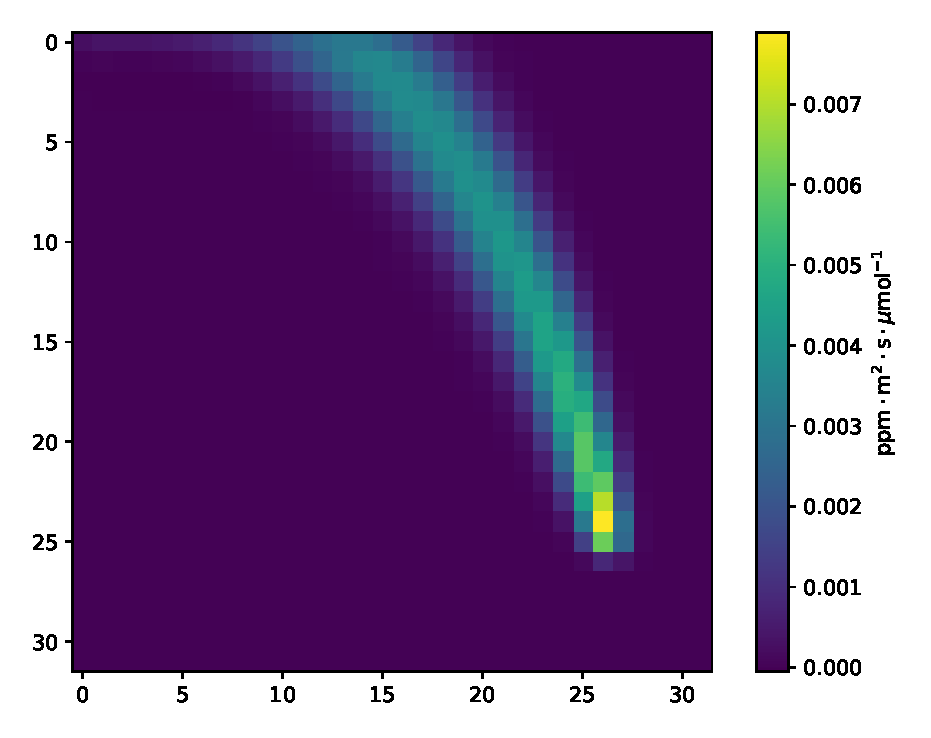
\includegraphics[width=0.6\textwidth]{figures/05_reconstruction/gaussian_plume_footprint.eps}
    \caption{Example Footprint Generated by Gaussian Plume Simulation}
    \label{fig:footprint}
\end{figure}

\textcite{UrbanSparseReconstruction} demonstrated that sensing matrices constructed using STILT \parencite{STILT} or the Gaussian plume model are both well suited for evaluating reconstruction quality in compressed sensing.
Given that STILT simulations are computationally expensive, we employ the Gaussian plume model to construct the footprints for the experiments.
Additionally, for some experiments, we utilize the footprints constructed using the Gaussian plume model by \textcite{UrbanSparseReconstructionFootprints} as they directly apply to our study.
It is important to note that our analysis uses the same footprints for all cities and that a static emission flux field is assumed during the measurement process.

\section{Inverse Problem Solvers}
This section goes over the implementation of the respective solvers, highlighting important hyperparameters.

\subsection{Sparse Reconstruction}
\subsubsection{Lasso}
The first type of sparse reconstruction solver uses \gls{Lasso} \parencite{Lasso}.
The \gls{Lasso} regularizer is computationally efficient, making it ideal for the Gaussian sensor matrix problem, which has $15360$ unknowns.
A grid search \parencite{HyperParameters} on the test data is used to tune the hyperparameter $\alpha$, which is set to $0.01$ for the test data.
This thesis uses the implementation from the scikit-learn library \parencite{sklearn}, which is based on the coordinate descent algorithm \parencite{CoordinateDescent}.

\subsubsection{Basis Pursuit}
The second type of sparse reconstruction solver is based on the \gls{BPDN} \parencite{BPDN} method, given that we are only concerned with noisy cases in this thesis.
The \gls{BPDN} solver is provided with the generated noise $\epsilon$ as input to determine the constraint factor $\delta = \norm{\epsilon}_2^2$, thus eliminating the need for hyperparameter tuning.
In combination with highly optimized solvers, \gls{BPDN} demonstrates superior results compared to the \gls{Lasso} regularizer.
However, due to the algorithmic complexity of the solvers, \gls{BPDN} is applied only in the atmospheric inversion case, where there are $1024$ unknowns.
The solver used for this task is the Gurobi solver \parencite{Gurobi}.

\subsubsection{Sparsity Transforms}
Since area sources are not inherently sparse, sparse reconstruction methods require a transformation to make the emission fields sparse.
In this thesis, two transforms inspired by \textcite{CSUsingAI} and \textcite{UrbanSparseReconstruction} are employed.
The first transform is the two-dimensional \gls{DWT}, specifically using Haar wavelets \parencite{Wavelets} and a third-level decomposition, following \textcite{UrbanSparseReconstruction}.
The PyWavelets library \parencite{PyWavelets} is used for this implementation.
The second transform applied is the two-dimensional \gls{DCT} \parencite{DCT}.
The SciPy library \parencite{SciPy} is used for this implementation.

The inverse problems are solved in the transformed bases, and the results are then inverse-transformed to the original domain.
For sector-wise reconstructions, transforms are applied per sector at the spatial level.

\subsection{Regularized Least Squares}
Following the approach of \textcite{UrbanSparseReconstruction}, this thesis also compares results to the \gls{LS} solver.
This solver addresses the following minimization problem: 
\begin{equation}
    \min \norm{x}_2 \quad \text{subject to} \quad  \norm{Ax -y}_2^2 \le \norm{\epsilon}_2^2
\end{equation}
Again, the Gurobi solver \parencite{Gurobi} is employed to solve this problem.
As with the \gls{BPDN} solver, the noise $\epsilon$ is assumed to be known and provided to the solver.
Due to computational limitations, this solver is only used in the atmospheric inversion case, where there are $1024$ unknowns.

\subsection{Generative Model}
For the solvers based on generative models, the generator $G$ must first be defined.
Let $D: \mathbb{R}^d \rightarrow \mathbb{R}^{32 \times 32 \times 15}$ represent the decoder of the \gls{VAE}.
Then, the generator $G: \mathbb{R}^d \rightarrow \mathbb{R}^{15360}$ is expressed as $G(z) = \vectorize(D(z))$, where the generator $G$ is simply the vectorization of the \gls{VAE}'s decoder.

In the case of atmospheric inversion, the generator is redefined as the sum of sectors $G_{\text{tot}}: \mathbb{R}^d \rightarrow \mathbb{R}^{1024}$:
\begin{equation}
    G_{\text{tot}}(z) = \vectorize\left(\sum_{i = 1}^{15}{D_i(z)}\right)
\end{equation}
where $D_i$ refers to the $i$-th sector of the generated emission field.
This implies that the model's output decomposes the emission field into individual sectors.
However, the solver's final output is the sum of these sectors.

\subsubsection{Generative Model Solver}
In this thesis, the generative model solver solves the following optimization problem:
\begin{equation}
    \min_{z}{\left( \norm{A G(z) - y}_2^2 \right)}
\end{equation}
without regularization, and it is solved numerically using the Adam optimizer \parencite{Adam}.
The absence of regularization is motivated by the observation that performance is better without it.

The initial latent variable $z_0 \in \mathbb{R}^d$ is sampled from a standard Gaussian distribution, $z_0 \sim \mathcal{N}(0, I)$.
The learning rate of the optimizer is tuned based on the observed optimization behavior, such as slow convergence or oscillations in the loss function. 
The maximum number of gradient update steps is set to $10,000$.
Alternatively, optimization stops early if no improvement in the objective function is seen for $250$ steps.

The solver tracks the best latent variable $z^\star$, and the final reconstructed solution is given by $\hat{x} = G(z^\star)$.

\subsubsection{Generative Model Solver With Sparse Offset}
The generative model solver with a sparse offset addresses the following optimization problem:
\begin{equation}
    \min_{z, s}{\left(\norm{s}_1 + \lambda \norm{A \left( G(z) + s \right) - y}_2^2 \right)}
\end{equation}
This problem is also solved using the Adam optimizer \parencite{Adam}.

The initial latent variable $z_0$ and the sparse offset $s_0$ are initialized as zero vectors.
A warmup optimization phase of $250$ steps is performed, during which the sparse offset $s$ is frozen, and only $z$ is updated.
The learning rate is set to $2 \cdot 10^{-2}$ during this warmup phase.
This warmup phase initially guides the optimization towards solutions within the generator's range.
After the warmup, the Adam optimizer updates both $z$ and $s$ simultaneously while keeping track of the best latent variable $z^\star$ and sparse offset $s^\star$.
The learning rate is adjusted as necessary by monitoring the optimization process.
The hyperparameter $\lambda$ must be tuned for each run, for instance, via grid search, based on the reconstruction loss $\norm{A \left( G(z) + s \right) - y}_2^2$.

The total number of optimization steps, including the warmup, is capped at $20,000$.
Again, the optimization terminates early if no improvement is observed for $250$ steps.
The final reconstructed solution is then the emission field $\hat{x} = G(z^\star) + s^\star$.
